\documentclass[a4paper,10pt]{article}
\usepackage[a4paper, total={180mm, 257mm}]{geometry}

\usepackage[colorlinks,linkcolor=blue,bookmarks,bookmarksopen,pdfauthor=krom]{hyperref}

\usepackage{fontspec}
\setmainfont[Path = fonts/, Extension = .ttf, BoldFont = ipagp]{ipamp}

\usepackage[compact]{titlesec}
\titlespacing{\section}{0em}{*0}{1.8em}
\titlespacing{\subsection}{0em}{*0}{2.3em}
\titlespacing{\subsubsection}{0em}{*0}{1.7em}
\titleformat{\section}{\normalfont\Huge}{\thesection}{0em}{}
\titleformat{\subsection}{\normalfont\Large}{\thesection}{0em}{}
\titleformat{\subsubsection}{\normalfont\normalsize}{\thesection}{0em}{}

\setlength\parindent{4em}
\setlength\parskip{0em}
\renewcommand{\baselinestretch}{1.24}

\usepackage{fancyhdr}
\pagestyle{fancy}
\fancyhf{}
\renewcommand\headrulewidth{0pt}

\usepackage{graphicx}
\graphicspath{{images/}}

\usepackage[usenames, dvipsnames]{color}
\definecolor{GTSgreen}{rgb}{0.35, 0.64, 0.18}

\begin{document}

\noindent\begin{picture}(0,0)
\put(186,-65){
\includegraphics[width=49mm]{GTSLogo}}
\put(186,-123){\color{GTSgreen}\Huge\textbf{\scalebox{2.85}[2.6]{GTS}}}
\put(125,-370){\Huge\scalebox{1.45}[1.45]{GTS 取扱説明書}}
\put(212,-397){\normalsize 2016 年 3 月 24 日}
\end{picture}

\newpage

\begin{center}
{\Huge{目次}}
\end{center}

\vspace{4.5em}

\noindent\LARGE インストール時設定\\[0.5em]
\large 01 \ スキャナーとドライバーの準備\\
02 \ TWAIN ドライバー環境設定 (※EPSON Scan Ver. 5.3.1.4 の場合)\\
03 \ 実行前設定 (※必要に応じて設定してください)\\[1.0em]
\LARGE 実行と終了\\[0.5em]
\large 04 \ 実行方法\\
05 \ 終了方法\\[1.0em]
\LARGE スキャン前の設定\\[0.5em]
\large 06 \ 解像度と回転と取り込む範囲の設定\\
07 \ 画像タイプの設定\\
08 \ 連番スキャンと保存ファイルの登録\\
09 \ 連番スキャンの確認\\
10 \ 連番スキャンの編集\\[1.0em]
\LARGE スキャン実行 \& 保存\\[0.5em]
\large 11 \ 連番スキャン (\&保存) の実行\\[1.0em]
\LARGE 状態保存と再スキャン\\[0.5em]
\large 12 \ 状態保存し、 作業の再現を可能にします\\
13 \ 作業を継続再開、 あるいは、 再スキャン等の作業を行うには\\[1.0em]
\LARGE トレース(フルカラー画像の 2 値化)\\[0.5em]
\large 14 \ トレースの準備\\
15 \ トレースの調整\\
16 \ トレースの実行保存\\[1.0em]
\LARGE フルカラースキャン \& トレース\\[0.5em]
\large 17 \ フルカラー画像のスキャンをしながら、 同時にトレースし保存するには\\
\\
付録 A 画像の表示変更方法

\fancyfoot[L]{\begin{picture}(0,0)
\put(0,0){
\includegraphics[width=25.8em, height=0.25em]{GTSFooter}}
\end{picture}
\vskip -0.3em \textbf{GTS}
}
\fancyfoot[R]{\vskip 0.1em \textbf{\thepage}}

\newpage

\renewcommand{\baselinestretch}{1.40}

\normalsize

\phantomsection
\section*{インストール時設定}
\addcontentsline{toc}{section}{インストール時設定}

\phantomsection
\subsection*{01 \ スキャナーとドライバーの準備}
\addcontentsline{toc}{subsection}{01 スキャナーとドライバーの準備}

\noindent TWAIN スキャナーをパソコンに接続し電源をいれます。\\
(EPSON DS-50000 , EPSON Scan Ver. 5.3.1.4 で動作確認しています。 その他については未確認です)\\
接続したスキャナーに対応した TWAIN ドライバーをインストールし、\\
動作することを確認してください。\\
TWAIN ドライバーは、 他のスキャナー機種用と混在せず、\\
単独でインストールします。\\

\phantomsection
\subsection*{02 \ TWAIN ドライバー環境設定 (※EPSON Scan Ver. 5.3.1.4 の場合)}
\addcontentsline{toc}{subsection}{02 TWAIN ドライバー環境設定 (※EPSON Scan Ver. 5.3.1.4 の場合)}

\noindent a “EPSON Scan" 実行し、 “EPSON Scan" ウインドウを開き、\par
\noindent\hskip 1.0em “環境設定 (O)..." ボタンをクリックし、 “環境設定" ウインドウを開きます\\
\\
b “プレビュー" タブをクリックし、\par
\noindent\hskip 1.0em “写真/フィルムの自動回転 (O)” のチェックを外します\\
\\
c “カラー" タブをクリックし、\par
\noindent\hskip 1.0em “常に自動露出を実行" のチェックを外します\par
\noindent\hskip 1.0em “ディスプレイガンマ" は “1.8" を選択します (必要に応じて他の値でもかまいません)\\
\\
d “書類" タブをクリックし、\par
\noindent\hskip 1.0em “境界補整量" をすべてゼロにします\\
\\
e “その他" タブをクリックし、\par
\noindent\hskip 1.0em “圧縮転送をする" のチェックを外します\\

\phantomsection
\subsection*{03 \ 実行前設定 (※必要に応じて設定してください)}
\addcontentsline{toc}{subsection}{03 実行前設定 (※必要に応じて設定してください)}

\phantomsection
\subsubsection*{○ “Level", “Load Config...", “Save As Config..." の初期フォルダー}
\addcontentsline{toc}{subsubsection}{○ “Level", “Load Config...", “Save As Config..." の初期フォルダー}

\noindent ファイル “gts\_install\_setup.txt" に記述します。\\
(このファイルは “gts.exe" の存在するフォルダーに置きます)\\
例えば、 “C:¥User¥public" を指定するなら、\\
browser\_directory\_path “C:¥User¥public"\\
と記入します。

\newpage

\noindent 指定がない場合 “C:¥" となります。\\

\phantomsection
\subsubsection*{○ 連番スキャン実行時のショートカットキーの設定}
\addcontentsline{toc}{subsubsection}{○ 連番スキャン実行時のショートカットキーの設定}

\noindent ファイル “gts\_install\_setup.txt" に記述します。\\
(このファイルは “gts.exe" の存在するフォルダーに置きます)\\
指定できるキーは Space, Enter, Esc のみです。\\
例えば、\\[-1.25em]

\setlength{\tabcolsep}{0em}
\renewcommand{\arraystretch}{1.0}
\noindent\begin{tabular}{p{17.0em}l}
short\_cut\_key\_start\_scan & Enter\\
short\_cut\_key\_rescan & Space\\
short\_cut\_key\_next\_scans & Enter\\
short\_cut\_key\_stop\_scan & Esc\\
\end{tabular}\\[-0.5em]

\noindent というように記入します。\\

\phantomsection
\subsubsection*{○ スキャンエリアのプリセット設定}
\addcontentsline{toc}{subsubsection}{○ スキャンエリアのプリセット設定}

\noindent ファイル “\_gts-scan\_area.txt" に記述します。\\
以下の場所のどこかに置きます。 上が優先度高くなります。\\[-1.25em]

\setlength{\tabcolsep}{0em}
\renewcommand{\arraystretch}{1.0}
\noindent\hskip 4.0em \begin{tabular}{p{13.0em}l}
各ユーザーのホーム & ※環境変数によるパス位置 → “\%HOMEDRIVE\%\%HOMEPATH\%"\\
全ユーザープロファイル & ※環境変数によるパス位置 → “\%ALLUSERSPROFILE\%"\\
共有のホーム & ※環境変数によるパス位置 → “\%PUBLIC\%"\\
\multicolumn{2}{l}{“gts.exe" の存在するフォルダー}\\
\end{tabular}\\[1.0em]

\noindent スキャンエリアの位置とサイズの指定\\
例えば、\\[-1.25em]

\setlength{\tabcolsep}{0em}
\renewcommand{\arraystretch}{1.0}
\noindent\begin{tabular}{p{8.5em}p{8.5em}p{8.5em}p{8.5em}l}
A3 & 0 & 0 & 43.18 & 29.718\\
NTSC\_in\_A3 & 1.778 & 0 & 39.624 & 29.718\\
HD\_in\_A3 & 0 & 2.714625 & 43.18 & 24.28875\\
\end{tabular}\\[-0.5em]

\noindent というように記入します。\\
\\
スキャンエリアの縦横比指定 (横固定で縦変化)\\
例えば、\\[-1.25em]

\setlength{\tabcolsep}{0em}
\renewcommand{\arraystretch}{1.0}
\noindent\begin{tabular}{p{8.5em}p{8.5em}p{8.5em}l}
aspect\_ratio & HD & 16 & 9\\
aspect\_ratio & NTSC & 4 & 3\\
\end{tabular}\\[-0.5em]

\noindent というように記入します。\\

\phantomsection
\subsubsection*{○ 再表示の位置と大きさ}
\addcontentsline{toc}{subsubsection}{○ 再表示の位置と大きさ}

\noindent ファイル “\_gts-desktop.txt" に記述します。\\
このファイルはログオンアカウントのホームフォルダーにあります。\\
アプリ終了時、自動保存します。

\newpage

\phantomsection
\section*{実行と終了}
\addcontentsline{toc}{section}{実行と終了}

\phantomsection
\subsection*{04 \ 実行方法}
\addcontentsline{toc}{subsection}{04 実行方法}

\noindent “gts.exe"\\
を実行します。

\noindent\begin{picture}(0,0)
\put(52,-237){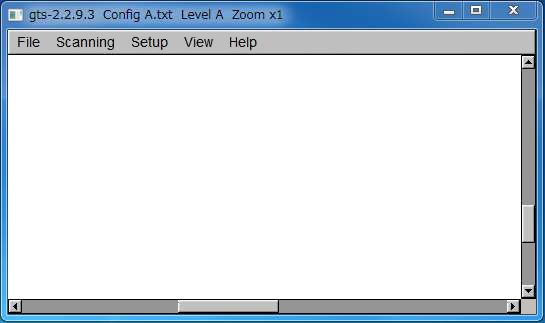
\includegraphics[width=143mm]{Config}}
\end{picture}\\[24.0em]

\noindent このとき、 「スキャナーとの正常な通信ができません、、、」\\
というメッセージを表示したら\\
・ スキャナーが接続されているか、\\
・ 電源スイッチが入っているか、\\
・ ドライバーが正しくインストールしてあるか、\\
等を再確認してください。\\

\phantomsection
\subsection*{05 \ 終了方法}
\addcontentsline{toc}{subsection}{05 終了方法}

\noindent “File" メニューから “Quit" を選択し、\\
表示した確認のダイオローグ画面で “Yes" をクリックすると終了します。\\
\\
“No" をクリックすると終了せず継続して作業できます。

\newpage

\phantomsection
\section*{スキャン前の設定}
\addcontentsline{toc}{section}{スキャン前の設定}

\phantomsection
\subsection*{06 \ 解像度と回転と取り込む範囲の設定}
\addcontentsline{toc}{subsection}{06 解像度と回転と取り込む範囲の設定}

\noindent “Setup" メニューの “Area and Rot90..." を選び\\
“Area and Rot90" ウインドウを開きます。

\noindent\begin{picture}(0,0)
\put(171,-216){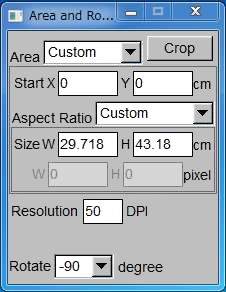
\includegraphics[width=59mm]{AreaAndRot90}}
\end{picture}\\[22.0em]

\noindent 以下、 「解像度」 → 「回転」 → 「取り込む範 囲」 の順に設定をします。\\

\phantomsection
\subsubsection*{○ 解像度}
\addcontentsline{toc}{subsubsection}{○ 解像度}

\noindent “Resolution" の入力部分をクリックし、\\
キーボードから数値入力します。\\
単位は Dot Per Inch です。\\
\\
“Crop" ボタンによるスキャンしたあとで、 解像度の変更をした場合、\\
“Crop" スキャンし直しが必要ですので注意してください。\\

\phantomsection
\subsubsection*{○ 回転}
\addcontentsline{toc}{subsubsection}{○ 回転}

\noindent 90 度単位で指定します。\\
“Rotate" のプルダウンから選んでください。\\

\phantomsection
\subsubsection*{○ 取り込む範囲}
\addcontentsline{toc}{subsubsection}{○ 取り込む範囲}

\noindent 設定方法は2つあり、プリセット設定と手動設定です。

\newpage

\noindent プリセット設定は、 あらかじめファイルに指定して、\\
“Area" の項目から選びます。\\
プリセットを設定するには\par
“03 実行前設定" → “○ スキャンエリアのプリセット設定"\\
を見てください。\\
\\
手動設定はスキャンしてみて絵を見ながら範囲を指定します。\\
“Crop" ボタンを押すと、 スキャナーの全範囲の絵をスキャンし、\\
画面に表示します。 同時に赤枠と小四角を表示します。\\
赤枠が範囲を示します。\\
小四角をマウス中ボタンでドラッグすることで範囲を変えます。\\
“Start X", “Y", “Size W", “H" の項目に数値を直接入力することもできます。\\
画像含めた全体の表示を変えるには\par
“付録 A 画像の表示変更方法"\\
を見てください。\\
\\
縦横比を指定の比にしたいなら “Aspect Ratio" プリセットを使用します。\\
プリセットを設定するには\par
“03 実行前設定" → “○ スキャンエリアのプリセット設定"\\
を見てください。\\
“Aspect Ratio" プリセットから選択すると、 横幅 “W" を固定した状態で、\\
高さ “H" 値が指定の比率に変わります。

\newpage

\phantomsection
\subsection*{07 \ 画像タイプの設定}
\addcontentsline{toc}{subsection}{07 画像タイプの設定}

\noindent “Setup" メニューの “Pixel Type and Bright..." を選び\\
“Pixel Type and Bright" ウインドウを開きます。

\noindent\begin{picture}(0,0)
\put(150,-152){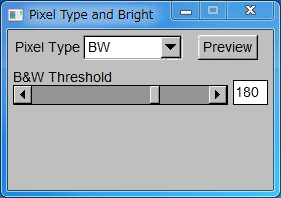
\includegraphics[width=73mm]{PixelTypeAndBright}}
\end{picture}\\[15.5em]

\phantomsection
\subsubsection*{○ 画像のタイプ “Pixel Type"}
\addcontentsline{toc}{subsubsection}{○ 画像のタイプ “Pixel Type"}

\noindent 以下の3種類から選択します。\\[-1.25em]

\setlength{\tabcolsep}{0em}
\renewcommand{\arraystretch}{1.0}
\begin{tabular}{p{8.5em}l}
BW & 白黒2値画像\\
Grayscale & 白黒諧調画像\\
RGB & フルカラー画像\\
\end{tabular}\\[1.0em]

\phantomsection
\subsubsection*{○ 取込調整}
\addcontentsline{toc}{subsubsection}{○ 取込調整}

\noindent “BW" の場合、スキャン時に、 直接白黒2値化します。\\
そのため、 白と黒の閾 (境界) 値を決めます。\\
“B\&W Threshold" に 0 から 255 の間の値で変化させ、\\
“Preview" ボタンでスキャンを繰り返すことで、 画像を確認しながら、\\
値を調整してください。\\
\\
“Grayscale", “RGB" の場合 “Brightness", “Contrast", “Gamma"\\
のパラメータがありますが、 基本的には、\\
全てデフォルト値を使うことをお勧めします。

\newpage

\phantomsection
\subsection*{08 \ 連番スキャンと保存ファイルの登録}
\addcontentsline{toc}{subsection}{08 連番スキャンと保存ファイルの登録}

\noindent “File" メニューの “Level..." を選び\\
“Browse Level" ウインドウを開く。

\noindent\begin{picture}(0,0)
\put(134,-351){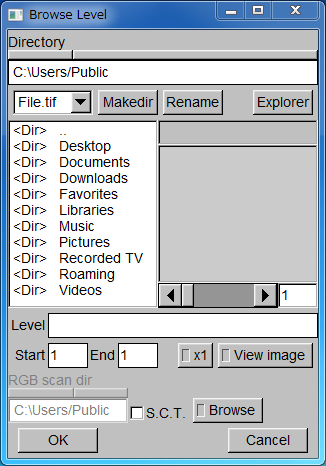
\includegraphics[width=85mm]{BrowseLevel}}
\end{picture}\\[34.0em]

\phantomsection
\subsubsection*{○ 連番画像の保存場所、 名前、 開始番号、 終了番号を設定}
\addcontentsline{toc}{subsubsection}{○ 連番画像の保存場所、 名前、 開始番号、 終了番号を設定}

\noindent 以下の項目、\\[-1.25em]

\setlength{\tabcolsep}{0em}
\renewcommand{\arraystretch}{1.0}
\begin{tabular}{p{8.5em}l}
“Directory" & 保存場所\\
“Level" & (ファイルの頭になる) 名前\\
“Start" & 開始 (フレーム) 番号\\
“End" & 終了 (フレーム) 番号\\
\end{tabular}\\[-0.5em]

\noindent に入力し、 “OK" ボタンをクリックします。\\
\\
“保存場所" を変えるには、\\
左に表示するリストからフォルダーをクリックして移動します。\\

\phantomsection
\subsubsection*{○ 新しいフォルダーを作成する場合}
\addcontentsline{toc}{subsubsection}{○ 新しいフォルダーを作成する場合}

\noindent “Makedir" ボタンを押して、 “New directory name" ダイオローグから、\\
フォルダー名をキーボード入力し、 “OK" ボタンをクリックします。

\newpage

\noindent\vspace{0.5em}

\phantomsection
\subsubsection*{○ フォルダーの名前を変更する場合}
\addcontentsline{toc}{subsubsection}{○ フォルダーの名前を変更する場合}

\noindent “Ctrl" キーを押しながら、 フォルダーをクリックし選択状態にします。\\
次に “Rename" ボタンを押して、 “Rename Directory" ダイオローグから、\\
フォルダー名を変更し、 “OK" ボタンをクリックします。\\

\phantomsection
\subsubsection*{○ フォルダー操作やファイル操作を行いたい場合}
\addcontentsline{toc}{subsubsection}{○ フォルダー操作やファイル操作を行いたい場合}

\noindent “Explorer" ボタンをクリックし、 Windows Explorer を開いてください。\\

\phantomsection
\subsubsection*{○ 保存ファイルの書式と拡張子}
\addcontentsline{toc}{subsubsection}{○ 保存ファイルの書式と拡張子}

\noindent 保存する画像ファイルの書式は TIFF です。\\
各ファイルは拡張子 “tif" が自動的に付きます。\\

\phantomsection
\subsubsection*{○ ファイル名の書式}
\addcontentsline{toc}{subsubsection}{○ ファイル名の書式}

\noindent 例えば、\\[-1.25em]

\setlength{\tabcolsep}{0em}
\renewcommand{\arraystretch}{1.0}
\begin{tabular}{p{8.5em}l}
“Level" & A\\
“Start" & 1\\
“End" & 2\\
\end{tabular}\\[-0.5em]

\noindent とすると、\par
“A.0001.tif”\par
“A.0002.tif”\\
という名前のファイル名に保存することになります。\\

\phantomsection
\subsubsection*{○ フルカラー画像の場合の中間ファイル名}
\addcontentsline{toc}{subsubsection}{○ フルカラー画像の場合の中間ファイル名}

\noindent ただし、 「画像タイプ」 で 「RGB」 を選んだ場合、\par
“A.0001.tif"\\
でなく、 名前に “\_full" を自動的に付加し、\par
“A\_full.0001.tif"\\
という名前で保存します。

\newpage

\phantomsection
\subsection*{09 \ 連番スキャンの確認}
\addcontentsline{toc}{subsection}{09 連番スキャンの確認}

\noindent “Setup" メニューの “File Number..." を選び\\
“Number"ウインドウを開く。

\noindent\begin{picture}(0,0)
\put(206,-283){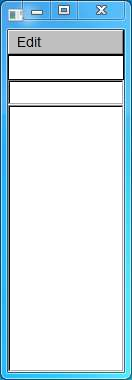
\includegraphics[width=34mm]{FileNumber}}
\end{picture}\\[28.0em]

\noindent “Level" によって設定した開始、 終了フレームの連番を表示し、\\
かつ、 選択状態であることを確認します。\\[2.0em]

\phantomsection
\subsection*{10 \ 連番スキャンの編集}
\addcontentsline{toc}{subsection}{10 連番スキャンの編集}

\noindent フレーム番号を削除するには、\\
“Number" ウインドウにて、 そのフレームのみ選択状態にし、\\
“Edit" メニューの “Delete" を選択すると、\\
選択状態のフレームを全て削除します。\\
\\
フレーム番号を追加するには、\\
“Number" ウインドウのメニューの直下にある入力エントリーをクリックし、\\
キーボードからその番号を入力し、 続けて Enter キー入力して追加します。\\
\\
連番を部分的にスキャンするときは、\\
そのフレーム番号のみ、 選択状態にします。

\newpage

\phantomsection
\section*{スキャン実行 \& 保存}
\addcontentsline{toc}{section}{スキャン実行 \& 保存}

\phantomsection
\subsection*{11 \ 連番スキャン (\&保存) の実行}
\addcontentsline{toc}{subsection}{11 連番スキャン (\&保存) の実行}

\noindent “Scanning" メニューの “Scan" を選ぶと即スキャンが始まります。

\noindent\begin{picture}(0,0)
\put(189,-74){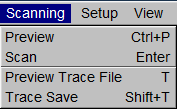
\includegraphics[width=46mm]{Scanning}}
\end{picture}\\[7.5em]

\noindent “Number" ウインドウで選択してある番号を上から順に、\\
スキャン\&保存し、 保存が済むと “S" マークが付きます。\\
\\
1枚目が終了すると、 “Next" ウインドウを表示します。

\noindent\begin{picture}(0,0)
\put(45,-100){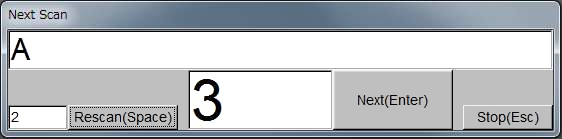
\includegraphics[width=148mm]{NextScan}}
\end{picture}\\[10.0em]

\noindent 各ボタンで次の動作をします。\\[-1.25em]

\setlength{\tabcolsep}{0em}
\renewcommand{\arraystretch}{1.0}
\begin{tabular}{p{8.5em}l}
“Rescan" & → 今の番号を再スキャンします\\
“Next" & → 次の番号のスキャンを実行します\\
“Stop" & → 連続スキャンを中止します\\
\end{tabular}\\[1.0em]

\noindent 最後の番号をスキャンしたあと “Next" ウインドウは表示しません。

\newpage

\phantomsection
\section*{状態保存と再スキャン}
\addcontentsline{toc}{section}{状態保存と再スキャン}

\phantomsection
\subsection*{12 \ 状態保存し、 作業の再現を可能にします}
\addcontentsline{toc}{subsection}{12 状態保存し、 作業の再現を可能にします}

\noindent “File" メニューの “Save As Config..." を選び\\
“Save As Config" ウインドウを開く。

\noindent\begin{picture}(0,0)
\put(145,-271){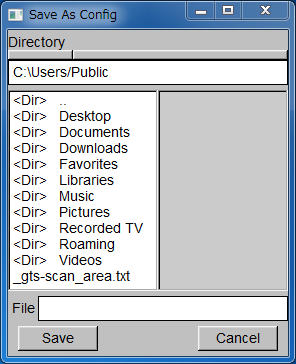
\includegraphics[width=78mm]{SaveAsConfig}}
\end{picture}\\[27.5em]

\noindent “Level" と同じ場所に移動し、 同じ名前をつけて “Save" で保存します。\\
\\
拡張子として “.txt" が自動的に付きます。\\
あえて “.txt" 指定しても2重に付くことはありません。

\newpage

\phantomsection
\subsection*{13 \ 作業を継続再開、 あるいは、 再スキャン等の作業を行うには}
\addcontentsline{toc}{subsection}{13 作業を継続再開、 あるいは、 再スキャン等の作業を行うには}

\noindent “File" メニューの “Load Config..." を選び\\
“Load Config" ウインドウを開く。

\noindent\begin{picture}(0,0)
\put(130,-278){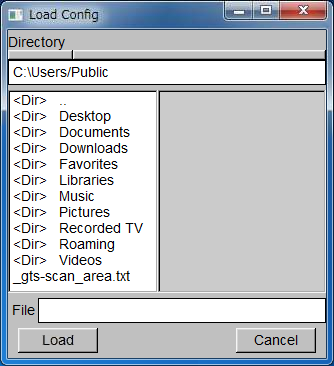
\includegraphics[width=88mm]{LoadConfig}}
\end{picture}\\[28.0em]

\noindent 保存しておいたファイルを選択し、 “Load" ボタンをクリック。\\
作業状態を再現します。

\newpage

\phantomsection
\section*{トレース (フルカラー画像の 2 値化)}
\addcontentsline{toc}{section}{トレース (フルカラー画像の 2 値化)}

\phantomsection
\subsection*{14 \ トレースの準備}
\addcontentsline{toc}{subsection}{14 トレースの準備}

\noindent まず、 フルカラー画像をスキャンしておきます。\\
\\
“File" メニューの “Level..." を選び\\
“Browse Level" ウインドウを開く。\\
\\
RGB 画像ファイルを以下の手順で指定します。\par
\noindent\hskip 1.0em 1 “Browse Level" の “Directory" 項目右下のプルダウン選択項目を、\par
\noindent\hskip 2.0em “Level.tif" にします。\par
\noindent\hskip 1.0em 2 スキャンした画像がある場所に移動し “Directory" にパスを設定します\par
\noindent\hskip 1.0em 3 画像ファイル名をクリックし、\par
\noindent\hskip 2.0em “Level", “Start", “End" の表示を確認する\par
\noindent\hskip 1.0em 4 “OK" ボタンをクリックし閉じる\par
\noindent\hskip 1.0em 5 “Number" ウインドウに番号と “S" が表示されていることを確認する\\
\\
画面に画像を表示します\\
“Scanning" メニューの “Preview Trace File" を選択すると\\
選択した番号の最初の画像を表示します。\\
なお、\\
画像の Zoom 値が 1/2 より小さいときは、2値化画像の再表示をしません\\
\\
画像全体の表示を変えるには\par
“付録 A 画像の表示変更方法"\\
を見てください。\\
\\
2値化以前の画像のみ表示する場合は、 “View" メニューの\\
“Color Trace Window" の中の、 “main\_to\_lr\_to\_sub" をクリックします。\\
元に戻すには同じ項目をもう一度クリックします。\\
\\
左右でなく、上下に分けて表示するには、 “View" メニューの\\
“Color Trace Window" の中の、 “lr\_to\_ud" をクリックします。\\
元に戻すには同じ項目をもう一度クリックします。\\

\newpage

\phantomsection
\subsection*{15 \ トレースの調整}
\addcontentsline{toc}{subsection}{15 トレースの調整}

\noindent “File" メニューの “Color Trace Enhancement..." を選び\\
“Color Trace Enhancement" ウインドウを開く。

\noindent\begin{picture}(0,0)
\put(140,-645){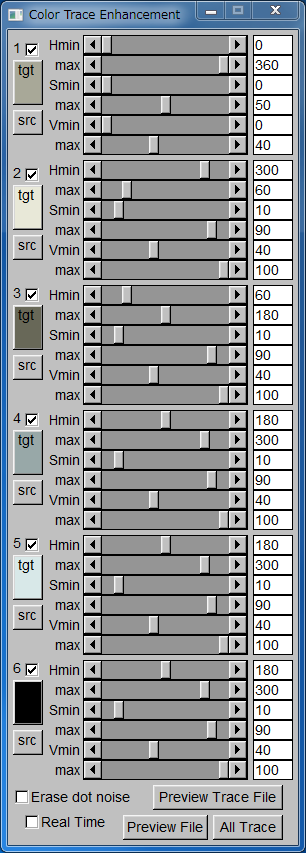
\includegraphics[width=81mm]{ColorTraceEnhancement}}
\end{picture}\\[28.0em]

\newpage

\noindent 以下、 画像を見ながら調整をします。\\
このとき、 Zoom を 1/2 以上にして、 さらに、\\
“Real Time" のチェックを入れておいてください。\\
\\
2 値化する色は、 1  から 6 まで6つの色まで指定できます。\\
\\
まず、 初期値として\par
全ての番号の、 右にあるチェックを入れる\par
Hmin, max, Smin, max, Vmin, max の各項目すべてゼロ\\
とします (1 から 6 まですべて)。\\
\\
もっとも出てほしい色から若い番号を使います。\\
例えば、\\[-1.25em]

\setlength{\tabcolsep}{0em}
\renewcommand{\arraystretch}{1.0}
\begin{tabular}{p{12.5em}l}
ハイライトの色線 & 赤鉛筆\\
黒線 & 鉛筆\\
影線 & 青鉛筆\\
\end{tabular}\\[1.0em]

\noindent の 3 色を 2 値化する場合\\
ハイライト線をもっとも重視し、 次に鉛筆線の順に 2 値化したいなら、\\
赤鉛筆は 1、 鉛筆は 2、 青鉛筆 3 を使います。\\
\\
2 値化した結果の色を設定します。\\
“tgt" ボタンをクリックして、 “Edit Color" ウインドウを表示し、

\noindent\begin{picture}(0,0)
\put(87,-107){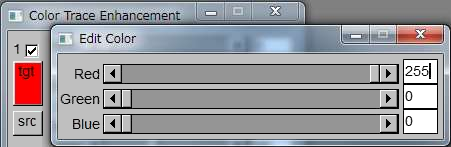
\includegraphics[width=118mm]{EditColor}}
\end{picture}\\[9.5em]

\noindent スライドバーで色を指定します。\\
\\
2 値化として拾う色の範囲を指定します。\par
赤鉛筆の調整例\\[-1.25em]

\setlength{\tabcolsep}{0em}
\renewcommand{\arraystretch}{1.0}
\hspace{4.0em}\begin{tabular}{rl}
Hmin \hspace{1.0em}  & 330\\
max \hspace{1.0em} & 30\\
Smin \hspace{1.0em} & 値を小さくすると線は太く、 大きくすると細くなる\\
max \hspace{1.0em} & 100\\
Vmin \hspace{1.0em} & 0\\
max \hspace{1.0em} & 100\\
\end{tabular}\\[-0.5em]

黒線の調整例\\[-1.25em]

\setlength{\tabcolsep}{0em}
\renewcommand{\arraystretch}{1.0}
\hspace{4.0em}\begin{tabular}{rl}
Hmin \hspace{1.0em} & 0\\
max \hspace{1.0em} & 360\\
\end{tabular}

\newpage

\setlength{\tabcolsep}{0em}
\renewcommand{\arraystretch}{1.0}
\hspace{4.0em}\begin{tabular}{rl}
Smin \hspace{1.0em} & 0\\
max \hspace{1.0em} & 100\\
Vmin \hspace{1.0em} & 0\\
max \hspace{1.0em} & 値を大きくすると線は太く、 小さくすると細くなる\\
\end{tabular}\\[-0.5em]

青鉛筆の調整例\\[-1.25em]

\setlength{\tabcolsep}{0em}
\renewcommand{\arraystretch}{1.0}
\hspace{4.0em}\begin{tabular}{rl}
Hmin \hspace{1.0em} & 210\\
max \hspace{1.0em} & 270\\
Smin \hspace{1.0em} & 値を小さくすると線は太く、 大きくすると細くなる\\
max \hspace{1.0em} & 100\\
Vmin \hspace{1.0em} & 0\\
max \hspace{1.0em} & 100\\
\end{tabular}\\[-0.5em]

\noindent ボタン説明\par
Erase dot noise\par
\hspace{4.0em} チェックを入れておくと、 1 ドットノイズを消します。\par
\hspace{4.0em} ゴミの点や、 線上の 1 ドット穴を自動でふさぎます。\par
Real Time\par
\hspace{4.0em} チェックを入れておくと、 数値の変化や、\par
\hspace{4.0em} スクロールするたびに、 2 値化画像を再表示します。\par
\hspace{4.0em} これは、 ズームが 1/4 以下の時は動作しません。\par
\hspace{4.0em} 1/2 以上にして使ってください。\par
Preview Trace File\par
\hspace{4.0em} “Number" ウインドウで選択した画像と\par
\hspace{4.0em} それを2値化した画像を再表示します。\par
Preview File\par
\hspace{4.0em} “Number" ウインドウで選択した画像のみを再表示します。\par
All Trace\par
\hspace{4.0em} 現在の画像から 2 値化画像を再表示します。\\

\phantomsection
\subsection*{16 \ トレースの実行保存}
\addcontentsline{toc}{subsection}{16 トレースの実行保存}

\noindent “Scanning" メニューの “Trace Save" を選択すると\\
ファイルを読み込み、 2 値化しながら保存します。\\
\\
途中キャンセルはできません。\\
\\
入力画像と同じ場所に保存します。\\
\\
入力画像が、 “A\_full.0001.tif" ならば、 “A.0001.tif" というファイル名で保存します。

\newpage

\phantomsection
\section*{フルカラースキャン \& トレース}
\addcontentsline{toc}{section}{フルカラースキャン \& トレース}

\phantomsection
\subsection*{17 \ フルカラー画像のスキャンをしながら、\\[0.75em]
\phantom{}\hspace{2.0em} 同時にトレースし保存するには}
\addcontentsline{toc}{subsection}{17 フルカラー画像のスキャンをしながら、 同時にトレースし保存するには}

\noindent “Browse Level" ウインドウの “S.C.T." (Save Color Trace level) にチェックを入れた状態で、\\
スキャンを実行すると2値化した画像も同時に保存します。\\
例えば、\\
フルカラー画像は “A\_full.0001.tif"\\
2値化画像は \hskip 1.9em “A.0001.tif"\\
というような名前で同じ場所に保存します。\\
\\
フルカラー画像を保存する場所を別に指定することができます。\\
まず、 “Browse Level" ウインドウの “RGB scan dir" の右の、\\
“Browse" ボタンをクリックし ON にします。\\
次に、 保存すべき場所に移動すると “RGB scan dir" のパスを変更します。\\
そして、 “OK" ボタンをクリックし閉じて、 スキャンを実行すると、\\
フルカラー画像のみ別指定の場所に保存します。

\newpage

\phantomsection
\subsection*{付録 A 画像の表示変更方法}
\addcontentsline{toc}{subsection}{付録 A 画像の表示変更方法}

\setlength{\tabcolsep}{0em}
\renewcommand{\arraystretch}{1.0}
\noindent\begin{tabular}{p{8.5em}l}
平行移動 & マウス中ボタンをドラッグ (小四角形がある場合その枠外)\\
拡大 & マウス左ボタン、 あるいは ‘z' キー\\
縮小 & マウス右ボタン、 あるいは ‘x' キー\\
全体表示 & ‘m' キー\\
ピクセル等倍 & ‘n' キー\\
\end{tabular}

\end{document}